\chapter{Methodology - CFD}
\label{chap:CFD}
    Uma forma muito utilizada para estudar sistemas granulares é a realização de simulações numéricas, que têm um papel importante na complementação das informações experimentais, o que aumenta ainda mais a compreensão dos fenômenos da física granular. Uma justificativa é o controle preciso dos parâmetros de entrada das simulações e do nível de complexidade acerca do objeto de estudo. Outra vantagem é a facilidade da medição próxima da escala dos grãos, como as cadeias de forças, até a escala do sistema, como o cisalhamento do material, evidenciando eventuais propriedades emergentes e suas causas.

    A técnica de simulação de materiais granulares que utilizamos neste trabalho é um \textit{DEM} conhecido na literatura como Dinâmica Molecular, ou \textit{Molecular Dynamics (MD)}. O método consiste em solucionar numericamente as equações de movimento quando aplicadas forças dinâmicas sobre os elementos a serem simulados. Uma vantagem deste método é que qualquer força que utilize parâmetros dentro da simulação e que possa ser descrita na interação com os elementos é aceita neste método.

    A técnica descrita no livro \textit{Computer Simulation of Liquids} \cite{Computer_Simulation_of_Liquids} utiliza-se dos formalismos da mecânica analítica através dos potenciais de interação entre os agentes, sejam potenciais lagrangianos, sejam potenciais hamiltonianos, para estabelecer a força que atua sobre cada agente. A desvantagem deste tipo de descrição é que forças dissipativas podem não aparecer, uma vez que a descrição das forças está relacionada diretamente com potenciais. Formalmente, o sistema deve obedecer ao conjunto de equações \ref{equ:lagrange} descritas pela função lagrangiana do sistema:
\begin{subequations}
    \label{equ:lagrange}
    \begin{empheq}[left={}]{align}
        \label{equ:lagrange1}
        \mathcal{L} &= \mathcal{T} - \mathcal{V},\\
        \label{equ:lagrange2}
        \sum_{k} \left[\frac{d}{dt} \left( \frac{\partial \mathcal{L}}{\partial \dot{q_k}} \right) - \left(\frac{\partial \mathcal{L}}{\partial q_k} \right)\right] &= 0,\\
        \label{equ:lagrange_forca}
        \vec{F}_{i} = \nabla \mathcal{L} &= -\nabla \mathcal{V},
    \end{empheq}
\end{subequations}
sendo que a notação descrita pelo conjunto de equações \ref{equ:lagrange}, $\mathcal{L}$ representa a função lagrangiana que rege a dinâmica do sistema, $\mathcal{T}$ a energia cinética, $\mathcal{V}$ a energia potencial, $k$ o número de coordenadas generalizadas do sistema, $q_{k}$ as coordenadas generalizadas, $\dot{q_{k}}$ as velocidades generalizadas, $\overrightarrow{F_{i}}$ a força exercida na partícula $i$ originada pelo gradiente do potencial $\mathcal{V}$.

    Já outras referências \cite{Dissertacao, Abraao-Dissertacao, Caio-Dissertacao, Caio-Tese, Bouzid-Tese, Wassgren-Tese, Felipe-Tese, Srdjan-Tese, Luding-Tese, Computational_Granular_Dynamics} utilizam o modelo diretamente das forças que agem sobre cada elemento.

\section{Equações de movimento}
    Para a realização da simulação, o conjunto de equações \ref{equ:movimento} deve ser satisfeito, o que leva em consideração as leis de Newton. Assim, tem-se a informação dos estados dos agentes em função do tempo.
\begin{subequations}
    \label{equ:movimento}
    \begin{empheq}[left={Translacional}\empheqlbrace]{align}
        \label{equ:posicao_linear}
        \vec{r}_{i}(t) &= \vec{r}_{i}(0) + \int_{0}^{t} \vec{v}_{i}(t) dt,\\
        \label{equ:velocidade_linear}
        \vec{v}_{i}(t) &= \vec{v}_{i}(0) + \int_{0}^{t} \vec{a}_{i}(t) dt,\\
        \label{equ:aceleracao_linear}
        \vec{a}_{i}(t) &= \sum_{j} \frac{\vec{F}_{i,j}(t)}{m_{i}},
    \end{empheq}
    \begin{empheq}[left={Rotacional}\empheqlbrace]{align}
        \label{equ:posicao_angular}
        \theta^{k}_{i}(t) &= \theta^{k}_{i}(0) + \int_{0}^{t} \vec{\omega}^{k}_{i}(t) dt,\\
        \label{equ:velocidade_angular}
        \vec{\omega}^{k}_{i}(t) &= \vec{\omega}^{k}_{i}(0) + \int_{0}^{t} \vec{\alpha}^{k}_{i}(t) dt,\\
        \label{equ:aceleracao_angular}
        \vec{\alpha}^{k}_{i}(t) &= {I^{k}_{i}}^{-1} \sum_{j} \vec{\tau}^{k}_{i,j}(t),
    \end{empheq}
\end{subequations}
em que $i$ é a i-ésima partícula do sistema, $\vec{r}_{i}(t)$ é o vetor de posição do centro de massa do corpo $i$ no instante de tempo $t$, $\vec{v}_{i}(t)$ ou $\vec{\dot{r}}_{i}(t)$ é o vetor de velocidade do centro de massa do corpo, $\vec{a}_{i}(t)$ ou $\vec{\dot{v}}_{i}(t)$ ou $\vec{\ddot{r}}_{i}(t)$ é o vetor de acelerações do centro de massa do corpo, $\vec{F}_{i,j}(t)$ é a componente da força que o centro de massa do corpo sofre por interagir com outro corpo ou campo $j$, $m_{i}$ é a massa do corpo, $\theta^{k}_{i}(t)$ é a base das coordenadas de rotação do corpo expressas na base $k$ do sistema, $\vec{\omega}^{k}_{i}(t)$ é o pseudovetor de velocidades angulares do corpo expressas na base $k$ do sistema, $\vec{\alpha}^{k}_{i}(t)$ é o pseudovetor de acelerações angulares do corpo, ${I^{k}_{i}}^{-1}$ é o inverso do tensor de inércia do corpo e $\vec{\tau}^{k}_{i,j}(t)$ é o vetor de torques que o corpo sofre por interagir com outro corpo ou campo. Lembrando que a relação entre o torque e a força que o causa pode ser descrita pela equação \ref{equ:torque}:
\begin{equation}
    \label{equ:torque}
    \vec{\tau}_{i,j}(t) = \vec{\chi}_{i,j}(t) \times \vec{F}_{i,j}(t),
\end{equation}
sendo que o vetor $\vec{\tau}_{i,j}(t)$ é o produto vetorial entre o vetor $\vec{\chi}_{i,j}(t)$, que liga o centro de massa da partícula $i$ ao ponto de aplicação da força, e o vetor $\vec{F}_{i,j}(t)$, o vetor da força causada por interagir com outro corpo ou campo $j$. As equações \ref{equ:aceleracao_linear} e \ref{equ:aceleracao_angular} expressam a segunda lei de Newton.

    A formulação descrita pelo conjunto de equações \ref{equ:movimento} abrange espaços em 1D, 2D e 3D, porém esta tese foca apenas na formulação de sistemas em 2D.

\subsection{Modelo de forças}
\label{subchap:Modelo_Forcas}
    As forças presentes nos sistemas modelados nesta tese incluem as forças de contato entre os agentes, que pertencem ao modelo reológico dos grãos, as forças de interação entre grão e fluido e a força gravitacional.

\subsubsection{Modelo reológico}
\label{subsubchap:Reologia}
    O modelo reológico dos agentes utilizado na simulação de \textit{MD} para materiais granulares foi proposto por Kelvin-Voigt \cite{Dissertacao}, com geometria circular pelos agentes. A reologia de Kelvin-Voigt modela a força de contato por uma mola e um amortecedor em paralelo na direção normal do contato, como exemplificado na figura \ref{fig:forcas}. A parcela da mola representa a contribuição elástica do material, relacionado com o módulo de Young, enquanto o amortecedor tem a função de atenuar a energia na colisão inelástica entre os grãos. Adicionalmente, um elemento parecido com uma mola é inserido na direção tangencial. Um modelo proposto em \cite{Caio-Tese} adiciona um elemento parecido com um amortecedor em paralelo à mola tangencial, modelando a resistência ao rolamento. Por causa da geometria circular, toda a variação de momento angular é causada pela força tangencial.

\begin{figure}
    \begin{minipage}{.45\linewidth}
        \centering
        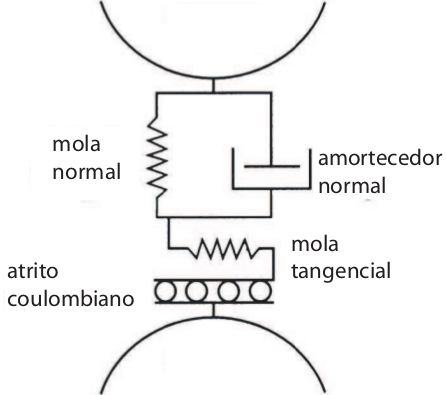
\includegraphics[width=0.9\textwidth]{04-figuras/Modelo_Forcas.png}
        \subcaption{Modelo de forças de contato entre os agentes.}
        \label{fig:forcas_modelo}
    \end{minipage}
    \begin{minipage}{.45\linewidth}
        \centering
        \includegraphics[width=0.9\textwidth]{04-figuras/Contato.tikz}
        \subcaption{Aplicação do contato entre os agentes.}
        \label{fig:forcas_contato}
    \end{minipage}
    \caption{Modelo de forças e a aplicação do contato entre os agentes. Figuras retiradas de \cite{Dissertacao}.}
    \label{fig:forcas}
\end{figure}

    Uma peculiaridade da \textit{MD} é a permissão de interpenetração entre os grãos, e portanto, neste modelo não há deformação no contato entre dois corpos. A interpenetração máxima é controlada pelo parâmetro de dureza do material e impondo penetração de $0.5\%$ dos raios.

    Para encontrar o valor da interpenetração $\delta$, na geometria circular, a equação \ref{equ:interpenetracao}:
\begin{equation}
    \label{equ:interpenetracao}
    \delta_{i,j}^{\perp} = \left(R_{i}+R_{j}-\left|\vec{r}_{j}-\vec{r}_{i}\right|\right)\mathcal{H}(R_{i}+R_{j}-\left|\vec{r}_{j}-\vec{r}_{i}\right|),
\end{equation}
em que $\delta_{i,j}^{\perp}$ é o valor da interpenetração entre os grãos $i$ e $j$, $R_{i}$ é o raio do corpo $i$, $R_{j}$ do corpo $j$, $\vec{r}_{i}$ é o vetor de posição do corpo $i$, $\vec{r}_{j}$ é o vetor de posição do corpo $j$ e $\mathcal{H}$ é a função de degrau de Heaviside. Então, quando a distância entre os corpos for maior que a soma dos raios, os corpos não estarão em contato e a função degrau de Heaviside indica que a interpenetração entre os grãos é nula.

    Com o contato entre os grãos, a consequência direta da interpenetração é o surgimento de uma força elástica repulsiva ao contato, e dependente da função de interpenetração $\delta^{\perp}$. A expressão da força pode ser calculada pela equação \ref{equ:forca_elastica}:
\begin{equation}
    \label{equ:forca_elastica}
    \vec{F}_{i,j}^{el} = -k_{n}\left(\delta_{i,j}^{\perp}\right)^{\frac{D}{2}}\hat{n}_{i,j},
\end{equation}
em que $\vec{F}_{i,j}^{el}$ é a força elástica que o corpo $i$ sente ao entrar em contato com o corpo $j$, $k_{n}$ é a constante relacionada a elasticidade do material na direção do contato, $\delta_{i,j}^{\perp}$ é a interpenetração entre os corpos $i$ e $j$, $D$ é a dimensão do sistema (no caso, $D=2$) e $\hat{n}_{i,j}$ é a direção normal do contato \cite{Dissertacao, Caio-Tese, Landau}. Pode-se escrever um potencial para esta força elástica como: $\mathcal{V} = \frac{1}{2}k_{n}{\delta_{i,j}^{\perp}}^2$.

    Associado à força elástica, também está presente a força de amortecimento. Por se tratar de uma força dissipativa, não se pode associar um potencial à força de amortecimento. A maior parcela da perda de energia dos materiais granulares está na colisão, e esta é a responsável. A equação \ref{equ:forca_amortecimento} descreve seu comportamento:
\begin{equation}
    \label{equ:forca_amortecimento}
    \vec{F}_{i,j}^{am} = -\gamma \left(\vec{v}_{i,j}.\hat{n}_{i,j}\right)\hat{n}_{i,j},
\end{equation}
em que $\vec{F}_{i,j}^{am}$ é a força de amortecimento que o corpo $i$ sente ao entrar em contato com o corpo $j$, $\gamma$ é a constante de amortecimento relacionada a inelasticidade da colisão, $\vec{v}_{i,j}$ é a velocidade relativa entre os centros de massa dos corpos $i$ e $j$ e e $\hat{n}_{i,j}$ é a direção normal do contato \cite{Dissertacao, Caio-Tese, Computational_Granular_Dynamics}.

    A constante de amortecimento está diretamente ligada ao coeficiente de restituição e pode ser utilizada equivalentemente através da transformação mostrada em \cite{Dissertacao}. Alguns autores utilizam o coeficiente de restituição nas simulações, como \cite{Computational_Granular_Dynamics, Luding-Tese, Srdjan-Tese}. Aqui, utilizaremos a constante de amortecimento.

    A força de atrito também está presente no modelo de simulação. Como as superfícies estão em contato, existirá uma força de atrito entre elas, se houver tendência de movimento uma em relação à outra. Em especial, devido à geometria circular, as forças de atrito agirão apenas na direção tangencial. A velocidade de deslocamento entre os pontos de contato dos corpos é dada pela equação \ref{equ:velocidade_relativa} a seguir:
\begin{equation}
  \label{equ:velocidade_relativa}
  \delta_{i,j}^{\parallel} = \vec{v}_{ij}.\hat{t}_{ij} - R_{i}\omega_{i} - R_{j}\omega_{j},
\end{equation}
em que $\delta_{i,j}^{\parallel}$ é a velocidade relativa entre os pontos de contato dos corpos $i$ e $j$, $\vec{v}_{ij}$ é a velocidade relativa entre os centros de massa dos corpos $i$ e $j$, $\hat{t}_{ij}$ é o vetor tangencial às superfícies de contato dos corpos $i$ e $j$, $R_{i}$ é o raio do corpo $i$, $R_{j}$ é o raio do corpo $j$, $\omega_{i}$ é a velocidade de rotação do corpo $i$ e $\omega_{j}$ é a velocidade de rotação do corpo $j$.

    Para a força tangencial, é necessário saber o deslocamento relativo dos pontos de contato, como dada pela equação \ref{equ:velocidade_relativa}, aplicados no sistema de equações \ref{equ:forca_atrito}, que modela a força de atrito com saturação, e é dada por:
\begin{equation}
    \label{equ:forca_atrito}
    \vec{F}_{i,j}^{at} = \left\{
    \begin{array}{l l l}
        \displaystyle -\int_{t_{0}}^{t_{f}} k_{t} \delta_{i,j}^{\parallel} \hat{t}_{ij}\, \mathrm{d} t, & \quad \textrm{se } k_{t} \left| \delta_{i,j}^{\parallel} \right| \leq \mu \left|F_{i,j}^{n}\right| & \textrm{ (Atrito Estático)} \\
        \displaystyle -\int_{t_{0}}^{t_{f}} \frac{\delta_{i,j}^{\parallel}}{\left|\delta_{i,j}^{\parallel}\right|} \mu \left| F_{i,j}^{n} \right| \hat{t}_{ij}\, \mathrm{d} t, & \quad \textrm{se } k_{t} \left| \delta_{i,j}^{\parallel} \right| > \mu \left| F_{i,j}^{n} \right| & \textrm{ (Atrito Cinético)}
    \end{array}
    \right.\ ,
\end{equation}
em que $\vec{F}_{i,j}^{at}$ é a força de atrito entre os corpos $i$ e $j$, $k_{t}$ é a constante elástica do material na direção tangencial, $\delta_{i,j}^{\parallel}$ é a velocidade relativa entre os pontos de contato dos corpos $i$ e $j$, $\hat{t}_{ij}$ é o vetor tangencial às superfícies de contato dos corpos $i$ e $j$, $\mu$ é o coeficiente de atrito entre as superfícies dos corpos $i$ e $j$ e $\vec{F}_{i,j}^{n} = \vec{F}_{i,j}^{el} +\vec{F}_{i,j}^{am}$ é a força normal às superfícies dos corpos $i$ e $j$.

\subsubsection{A força externa: Gravidade}
\label{subsubchap:Gravidade}
    Para este modelo, a influência gravitacional é aproximada por uma constante, já que a simulação não leva em conta que a influência da massa dos corpos é muito pequena, se comparada com a massa do planeta em que está situada a simulação, bem como a variação de altura do sistema simulado é muito pequeno e está próximo à superfície do planeta, quando comparada com o raio do planeta. Por conveniência, normalizamos a gravidade como valor unitário.

\subsubsection{As forças do fluido}
\label{subsubchap:Fluido}
    A força que o fluido exerce sobre os corpos pode ser entendida como contribuição de diferentes modelos e casos. Uma formulação mais detalhada sobre cada parcela de forças que o fluido exerce sobre cada corpo é descrita pela equação \ref{equ:forcas_fluido}:
\begin{equation}
    \label{equ:forcas_fluido}
    \vec{F}_{i}^{Fluid} = \vec{F}_{i}^{Arch} +\vec{F}_{i}^{Drag} +\vec{F}_{i}^{Magnus} +\vec{F}_{i}^{Lift} +\vec{F}_{i}^{AddedMass} +\vec{F}_{i}^{Basset},
\end{equation}
em que $\vec{F}_{i}^{Fluid}$ é a contribuição total das forças que o fluido exerce sobre o corpo $i$, $\vec{F}_{i}^{Arch}$ é a força de Arquimedes sobre o corpo $i$, $\vec{F}_{i}^{Drag}$ é a força de arrasto sobre o corpo $i$, $\vec{F}_{i}^{Magnus}$ é a força de Magnus sobre o corpo $i$, $\vec{F}_{i}^{Lift}$ é a força de sustentação sobre o corpo $i$, $\vec{F}_{i}^{AddedMass}$ é a força de adição de massa sobre o corpo $i$ e $\vec{F}_{i}^{Basset}$ é a força histórica de Basset sobre o corpo $i$. Como simplificação do modelo, utilizaremos apenas as forças de Arquimedes e as forças de arraste do fluido \cite{Fluid_Mechanics, Numerical_simulation_of_turbulent_sediment_transport, Maurin-Tese}.

    A força de Arquimedes pode ser escrita como na equação \ref{equ:arquimedes}, enquanto a força de arraste pode ser escrita como na equação \ref{equ:arraste}:
\begin{equation}
    \label{equ:arquimedes}
    \vec{F}_{i}^{Arch} = \frac{\pi}{6} d_{i}^{3} \vec{\nabla}.\overline{\overline{\sigma}},
\end{equation}
em que $\vec{F}_{i}^{Arch}$ é a força de Arquimedes no corpo $i$, $d_{i}$ é o diâmetro do corpo $i$ e $\vec{\nabla}.\overline{\overline{\sigma}}$ é o divergente do tensor de tensão do fluido $\overline{\overline{\sigma}}$, e:
\begin{equation}
    \label{equ:arraste}
    \vec{F}_{i}^{Drag} = \frac{\pi}{8}\rho_{f}d_{i}^{2}C_{d}(\mathcal{R}_{u})\left|\vec{u}_{f}-\vec{v}_{i}\right|(\vec{u}_{f}-\vec{v}_{i}),
\end{equation}
em que $\vec{F}_{i}^{Drag}$ é a força de arraste no corpo $i$, $\rho_{f}$ é a densidade do fluido, $d_{i}$ é o diâmetro do corpo $i$, $C_{d}(\mathcal{R}_{u})$ é o coeficiente de arrasto em função do número de Reynolds do corpo, descrito pela equação \ref{equ:reynolds_arraste}, $\vec{u}_{f}$ é a velocidade do fluido, $\vec{v}_{i}$ é a velocidade do corpo \cite{Numerical_simulation_of_turbulent_sediment_transport}.

\begin{equation}
    \label{equ:reynolds_arraste}
    C_{u}(\mathcal{R}_{u}) = \left( \sqrt{C_{d}^{\infty}} +\sqrt{\frac{\mathcal{R}_{u}^{c}}{\mathcal{R}_{u}}} \right)^{2}
\end{equation}
em que $C_{u}(\mathcal{R}_{u})$ é o coeficiente de arrasto em função do número de Reynolds do corpo, $C_{d}^{\infty} \simeq 0.5$ é o coeficiente de arrasto do grão no limite turbulento ($\mathcal{R}_{u} \to \infty$), $\mathcal{R}_{u}^{c} \simeq 24$ é o número de Reynolds de transição do corpo na qual o coeficiente de arrasto torna-se quase constante e a equação \ref{equ:reynolds_fluido_grao} que relaciona o número de Reynolds do corpo com os parâmetros do sistema:
\begin{equation}
    \label{equ:reynolds_fluido_grao}
    \mathcal{R}_{u} = \frac{d_{i}}{\nu} \left| \vec{u}_{f} -\vec{v}_{i} \right|
\end{equation}
em que $d_{i}$ é o diâmetro do corpo $i$, $\nu$ é a viscosidade dinâmica do sistema, $\vec{u}_{f}$ é a velocidade do fluido e $\vec{v}_{i}$ é a velocidade do corpo $i$ \cite{Numerical_simulation_of_turbulent_sediment_transport}.

\subsection{O modelo do fluido}
    Para o fluido, a equação geral que rege o sistema é a equação de Navier-Stokes, que é a aplicação da segunda lei de Newton para a massa específica em meios contínuos e a aplicação das leis de conservação de massa e de momento \cite{Physical_Hydrodynamics, Fluid_Mechanics}. Para a equação da conservação de massa, temos a equação \ref{equ:conservacao_massa}:
\begin{equation}
    \label{equ:conservacao_massa}
    \frac{\partial \rho^{f}}{\partial t} +\vec{\nabla}.(\rho \vec{u}^{f}) = 0,
\end{equation}
em que $\rho^{f}$ é a densidade do fluido, e $\vec{u}^{f}$ é a velocidade do fluido.

    A equação \ref{equ:conservacao_momento} descreve a conservação do momento como:
\begin{equation}
    \label{equ:conservacao_momento}
    \frac{\partial}{\partial t}\left(\rho^{f}\vec{u}^{f}\right) +\vec{\nabla}.\left(\rho^{f}\vec{u}^{f}\otimes\vec{u}^{f}\right) = \overline{\overline{\sigma}} +p_{ext},
\end{equation}
em que $\rho^{f}$ é a densidade do fluido, $\vec{u}^{f}$ é a velocidade do fluido, $\overline{\overline{\sigma}}$ é o tensor tensão do fluido e $p_{ext}$ é a pressão causada por agentes externos, como a gravidade e as forças dos corpos que interagem com o fluido.

    Na formulação da conservação do momento, existe internamente a conservação da massa, e se escrevermos os termos da equação efetuando-se os produtos internos e as derivadas, teremos a equação \ref{equ:Navier-Stokes}, que é a equação de Navier-Stokes:
\begin{equation}
    \label{equ:Navier-Stokes}
    \rho^{f} \frac{\partial \vec{u}^{f}}{\partial t} +\rho^{f}\left(\vec{u}^{f}.\vec{\nabla}\right)\vec{u}^{f} = \vec{\nabla}.\overline{\overline{\sigma}} +p_{ext},
\end{equation}
em que $\rho^{f}$ é a densidade do fluido, $\vec{u}^{f}$ é a velocidade do fluido, $\overline{\overline{\sigma}}$ é o tensor tensão do fluido e $p_{ext}$ é a pressão causada por agentes externos e que o tensor tensão do fluido pode ser escrito em função das pressões internas e do cisalhamento do fluido, como na equação \ref{equ:tensor_tensao}:
\begin{equation}
    \label{equ:tensor_tensao}
    \overline{\overline{\sigma}} = \left(
    \begin{matrix}
        \sigma_{xx} & \tau_{xy} \\
        \tau_{yx} & \sigma_{yy}
    \end{matrix}
    \right),
\end{equation}
em que $\overline{\overline{\sigma}}$ é o tensor de tensão do fluido, $\sigma$ são as componentes de tensão e a pressão do fluido é $p=-\frac{1}{2}(\sigma_{xx}+\sigma_{yy})$, e $\tau$ são as componentes do cisalhamento do fluido, sendo que $\tau_{xy} = \tau{yx}$, indicando que são simétricas.

    Uma importante medida é a taxa de deformação do fluido, dada pela equação \ref{equ:taxa_deformacao}:
\begin{equation}
    \label{equ:taxa_deformacao}
    \dot{\gamma}_{xy} = \frac{1}{2} \left(\frac{\partial u_{x}}{\partial y} +\frac{\partial u_{y}}{\partial x} \right),
\end{equation}
em que $\dot{\gamma_{xy}}$ e $\dot{\gamma_{yx}}$ são as componentes do tensor da taxa de deformação, $u_{x}$ é a velocidade do fluido na direção de escoamento e $u_{y}$ é a velocidade do fluido na direção da gravidade. As componentes $\dot{\gamma_{xy}}$ e $\dot{\gamma_{yx}}$ são simétricas, sendo também equivalentes às componentes cruzadas do divergente do campo de velocidades.

    O cisalhamento do fluido controla algumas características do fluido, como por exemplo o regime de escoamento. A equação que rege o cisalhamento é a equação \ref{equ:cisalhamento}:
\begin{equation}
    \label{equ:cisalhamento}
    \tau = \rho^{f}(\nu+\nu_{t})\dot{\gamma},
\end{equation}
em que $\tau$ é cisalhamento do fluido, $\rho^{f}$ é a densidade do fluido, $\nu$ é a viscosidade intrínseca do fluido, $\nu_{t}$ é a viscosidade que insere turbulência no fluido e $\dot{\gamma}$ é o tensor da taxa de deformação do fluido e é descrito pela equação \ref{equ:taxa_deformacao}. Para que o escoamento seja laminar em um fluido newtoniano, o termo de viscosidade turbulenta deve ser nulo.

    As considerações feitas sobre o fluido são que o fluido é incompressível, que o fluido não circula na direção da gravidade (direção $x$ de escoamento), que possui condição periódica de contorno na direção de escoamento, ou seja, o que acontece de um lado do sistema é o mesmo que acontece no outro e o volume ocupado pelo fluido é o todo o volume não ocupado pelos corpos. As implicações destas condições simplificam as equações \ref{equ:conservacao_massa}, \ref{equ:conservacao_momento} e \ref{equ:Navier-Stokes}. No caso da conservação da massa a implicação da incompressibilidade do fluido é a conservação do volume ao longo de todo o tempo e todo o espaço. Já a condição periódica de contorno na direção do escoamento, em relação à  Navier-Stokes, equação \ref{equ:Navier-Stokes}, implica que a tensão na direção de escoamento seja nula, ou seja, $\sigma_{xx} = 0$ quando não houverem corpos. Para o fluido não circular na direção da gravidade, toda a camada de escoamento é tomada por uma média na direção do escoamento (direção $x$). Portanto, a simplificação do tensor de tensões do fluido resume-se na equação \ref{equ:divergente_tensor_tensao}:
\begin{equation}
    \label{equ:divergente_tensor_tensao}
    \vec{\nabla}.\overline{\overline{\sigma}} = \frac{\partial \tau}{\partial y} \hat{x} - \frac{\partial p}{\partial y} \hat{y}
\end{equation}
em que $\overline{\overline{\sigma}}$ é o tensor de tensão do fluido, $\tau$ é a componente do cisalhamento do fluido, $p$ é componente da pressão do fluido, $\hat{x}$ é a direção de escoamento do fluido e $\hat{y}$ é a direção da gravidade.

    Aplicando as considerações feitas sobre o fluido na equação de Navier-Stokes, equação \ref{equ:Navier-Stokes}, tem-se o sistema de equações em relações às direções de escoamento do fluido ($x$) e da gravidade ($y$) iguais a:
\begin{subequations}
    \label{equ:fluido}
    \begin{empheq}[left={}\empheqlbrace]{align}
        \label{equ:fluido_x}
        (1-\phi) \rho^{f} \frac{\partial u_{x}^{f}}{\partial t} &= (1-\phi) \frac{\partial \tau}{\partial y} - p_{x}^{body} & : \hat{x},\\
        \label{equ:fluido_y}
         0 &= -(1-\phi) \frac{\partial \sigma_{yy}}{\partial x} - p_{y}^{body} + (1-\phi)\rho^{f}g & : \hat{y},
    \end{empheq}
\end{subequations}
em que $\rho^{f}$ é a densidade do fluido, $u_{x}^{f}$ é a componente da velocidade na direção do escoamento, $\phi$ é o coeficiente de compactação dos corpos, $\tau$ é a componente do cisalhamento do fluido, $\sigma_{yy}$ é a componente da tensão no fluido, $p_{x}^{body}$ é a pressão que os corpos fazem sobre a direção de escoamento $x$, $p_{y}^{body}$ é a pressão que os corpos fazem sobre a direção gravitacional $y$ e $g$ é o valor da gravidade.

    Para a taxa de deformação do fluido, a aplicação das considerações do fluido resulta na equação \ref{equ:taxa_deformacao_final}:
\begin{equation}
    \label{equ:taxa_deformacao_final}
    \dot{\gamma_{xy}} = \frac{\partial u_{x}}{\partial y},
\end{equation}
em que $\dot{\gamma_{xy}}$ é a componente do tensor da taxa de deformação, $u_{x}$ é a velocidade do fluido na direção de escoamento e $y$ é a direção da gravidade.

    Existem vários modelos de turbulência para serem abordados em um fluido. Neste trabalho escolhemos o modelo de turbulência de Prandtl e o termo viscosidade turbulenta apresenta-se como na equação \ref{equ:viscosidade_turbulenta}:
\begin{equation}
    \label{equ:viscosidade_turbulenta}
    \begin{array}{l}
        \nu_{t} = l^2\left|\dot{\gamma}\right|, \textrm{ou seja,} \\
        \nu_{t} = l^2\left|\frac{\partial u_{x}}{\partial y}\right|,
    \end{array}
\end{equation}
em que $\nu_{t}$ é o modelo da turbulência, $l$ é um comprimento característico da turbulência e da vorticidade, $\dot{\gamma}$ é a taxa de deformação do fluido, $u_{x}$ é a velocidade do fluido na direção de escoamento e $y$ é a direção da gravidade.

    O cisalhamento do fluido controla algumas características do fluido, como por exemplo o regime de escoamento. A equação que rege o cisalhamento é a equação \ref{equ:cisalhamento}:
\begin{equation}
    \label{equ:cisalhamento}
    \tau = \rho^{f}\left(\nu+l^{2}\left|\frac{\partial u_{x}}{\partial y}\right|\right)\frac{\partial u_{x}}{\partial y},
\end{equation}
em que $\tau$ é cisalhamento do fluido, $\rho^{f}$ é a densidade do fluido, $\nu$ é a viscosidade intrínseca do fluido, $l^{2}\left|\frac{\partial u_{x}}{\partial y}\right|$ é a viscosidade que insere o efeito médio da turbulência no fluido e $\frac{\partial u_{x}}{\partial y}$ é o tensor da taxa de deformação do fluido e é equivalente à equação \ref{equ:taxa_deformacao}. Para que o escoamento seja laminar em um fluido newtoniano, o termo de viscosidade turbulenta deve ser nulo.

    Para a mistura do fluido e do granular, tomamos o comprimento característico da turbulência sempre acima das camadas estáticas do material granular, e portanto assumimos o comportamento descrito pela equação \ref{equ:comprimento_turbulencia} do comprimento característico da turbulência proposto por van Driest \cite{Numerical_simulation_of_turbulent_sediment_transport}:
\begin{subequations}
    \label{equ:comprimento_turbulencia}
    \begin{empheq}[left={l(y_{b}) =}\empheqlbrace]{align}
        \label{equ:comprimento_turbulencia_granular}
        & 0 & \textrm{se } y \leq y_{b}, \\
        \label{equ:comprimento_turbulencia_fluido}
        & \kappa (y -y_{b})\left[1-e^{-\left(y -y_{b}\right)\frac{u_{*}}{\nu \mathcal{R}_{vD}}} \right] & \textrm{se } y > y_{b},
    \end{empheq}
\end{subequations}
em que $l(y_{b})$ é o comprimento característico da turbulência, $\kappa \simeq 0,4$ é a constante de von Karman, $y$ é a altura do fluido, $y_{b}$ é a posição do topo da camada dos sólidos não transportados, $u_{*}$ é a velocidade característica de cisalhamento imposta no topo do fluido, $\nu$ é a viscosidade do fluido e $\mathcal{R}_{vD} \simeq 26$ é o número Reynolds de van Driest \cite{Numerical_simulation_of_turbulent_sediment_transport}. Porém outros comprimentos característicos da turbulência foram levados em consideração e estão descritos nas referências \cite{Numerical_simulation_of_turbulent_sediment_transport, Maurin-Tese}.

\subsection{Discretização temporal}
    Para a simulação computacional dos corpos sólidos, as equações da cinemática devem ser reescritas como expansões da série de Taylor, interpolando o sistema de equações de velocidade pelo algoritmo conhecido como \textit{Velocity Verlet} \cite{Verlet, Computer_Simulation_of_Liquids}. As equações de movimento discretizadas no tempo, em função do passo de tempo $\Delta t$, tornam-se como no conjunto de equações \ref{equ:movimento_discreto}:
\begin{subequations}
    \label{equ:movimento_discreto}
    \begin{empheq}[left={Translacional}\empheqlbrace]{align}
        \label{equ:posicao_linear_discreta}
        {\vec{r}_{i}}^{\;n+1} &= {\vec{r}_{i}}^{\;n} + {\vec{v}_{i}}^{\;n} \Delta t + \frac{{\vec{a}_{i}}^{\;n}}{2} (\Delta t)^{2},\\
        \label{equ:velocidade_linear_discreta}
        {\vec{v}_{i}}^{\;n+1} &= {\vec{v}_{i}}^{\;n} + \frac{{\vec{a}_{i}}^{\;n}+{\vec{a}_{i}}^{\;n+1}}{2} \Delta t,\\
        \label{equ:aceleracao_linear_discreta}
        {\vec{a}_{i}}^{\;n+1} &= \frac{\sum_{j} {\vec{F}_{i,j}}^{\;n+1} + \sum {\vec{F}_{i,ext}}^{\;n+1}}{m_{i}},
    \end{empheq}
    \begin{empheq}[left={Rotacional}\empheqlbrace]{align}
        \label{equ:posicao_angular_discreta}
        {\theta_{i}}^{n+1} &= {\theta_{i}}^{n} + {\vec{\omega}_{i}}^{\;n} \Delta t + \frac{{\vec{\alpha}_{i}}^{\;n}}{2} (\Delta t)^{2},\\
        \label{equ:velocidade_angular_discreta}
        {\vec{\omega}_{i}}^{\;n+1} &= {\vec{\omega}_{i}}^{\;n} +\frac{{\vec{\alpha}_{i}}^{\;n}+{\vec{\alpha}_{i}}^{\;n+1}}{2} \Delta t,\\
        \label{equ:aceleracao_linear_discreta}
        {\vec{\alpha}_{i}}^{\;n+1} &= {I_{i}}^{-1} \sum_{j} {\vec{\tau}_{i,j}}^{\;n},
    \end{empheq}
\end{subequations}
em que $i$ é o índice do corpo que movimenta, $j$ é o índice do corpo em contato com o corpo $i$, $n$ é o passo de tempo, $\vec{r}$ é a posição do corpo, $\vec{v}$ é a velocidade do corpo, $\vec{a}$ é a aceleração do corpo, $\Delta t$ é o tamanho do passo de tempo, $\vec{F}_{i,j}$ é a força de contato entre os corpos $i$ e $j$, $\vec{F}_{ext}$ são as forças externas, como gravidade e força que o fluido exerce sobre o corpo, $m$ é a massa do corpo, $\theta$ é a posição angular do corpo, $\vec{\omega}$ é a velocidade angular do corpo, $\vec{\alpha}$ é a aceleração angular do corpo, $\vec{\tau}$ é o torque sobre o corpo, $I$ é o momento de inércia do corpo.

    O conjunto de equações \ref{equ:movimento_discreto} está escrito para o sistema 2D, uma vez que só há um grau de liberdade para a rotação, e consequentemente todas as equações passam a ser escritas em função de um único parâmetro. A aproximação da velocidade como a ponderação entre as acelerações no instante de tempo atual e futuro é a chave para a minimização da imprecisão gerada pela discretização \cite{Computer_Simulation_of_Liquids}.

    Para o fluido, discretizamos a equação \ref{equ:fluido_x} de forma explícita\footnote{A forma explícita de resolução de um método de equações de diferenças resolve o sistema para o próximo passo de tempo com as operações originais da equação diferencial. Toda a discretização é feita sobre as funções do passo de tempo atual resultando no passo de tempo posterior. A desvantagem desta técnica é o fator de instabilidade da solução que pode vir a ocorrer. A vantagem é que o sistema sempre pode ser escrito por estas equações.}. Por causa da não linearidade das equações no termo de turbulência, ainda não conseguimos escrever uma expressão implícita\footnote{A forma implícita de resolução de um método de equações de diferenças resolve o sistema do próximo passo de tempo com base nas raízes da equação diferencial do problema. Toda a discretização é feita considerando as raízes que solucionam a equação. A desvantagem desta técnica é o fato de nem sempre existir algoritmo que encontre as raízes. A vantagem é que o fator de estabilidade é mais permissivo.} para este sistema. Alguns livros tratam exclusivamente o assunto da discretização da equação de difusão linear e estão referenciados em \cite{Transferencia_de_calor_e_mecanica_dos_fluidos_computacional, Numerical_Methods_for_Scientists_and_Engineers, Numerical_Recipes, Numerical_Solution_of_Partial_Differential_Equations}. A equação para o fluido, em sua forma discretizada torna-se então o sistema de equações \ref{equ:fluido_discreto}:
\begin{subequations}
    \label{equ:fluido_discreto}
    \begin{empheq}[left={}\empheqlbrace]{align}
        \label{equ:fluido_discreto_velocidade}
        {u_{x}}_{\;k}^{n+1} &= {u_{x}}_{\;k}^{\;n} + \frac{\Delta t}{\rho^{f}\Delta y} \left[\tau_{\;k}^{\;n} -\tau_{k-1}^{\;n}\right] - \frac{\Delta t}{\rho^{f}}{P}_{\;k}^{\;n}, \\
        \label{equ:fluido_discreto_cisalhamento}
        \tau_{\;k}^{\;n} &= \rho^{f} \left[\nu +{l_{k}}^{2}\left|\frac{{u_{x}}_{k+1}^{\;n}-{u_{x}}_{\;k}^{\;n}}{\Delta y}\right|\right]\left(\frac{{u_{x}}_{k-1}^{n}-{u_{x}}_{\;k}^{\;n}}{\Delta y}\right),
    \end{empheq}
\end{subequations}
em que $k$ é o índice discretização espacial do fluido, $n$ é o passo de tempo, $u_{x}$ é a velocidade de escoamento do fluido, $\Delta y$ é o espaçamento da malha do fluido, $\Delta t$ é o intervalo entre os passos de tempo, $\rho^{f}$ é a densidade do fluido, $\tau$ é o cisalhamento do fluido, $P$ é a pressão que os corpos sólidos fazem no fluido, $\nu$ é a viscosidade do fluido e $l$ é o comprimento característico da turbulência.

\section{Algoritmo}
    Além das equações que regem o sistema, uma série de procedimentos devem ser realizados para que a simulação possa ocorrer. Cada um destes passos são essenciais para que a simulação ocorra, e são dependentes uns dos outros. O algoritmo \ref{alg:MD} determina as rotinas para a execução da simulação. Utilizamos o \textit{Gear Predictor-Corrector} de 3ª ordem com o \textit{Velocity Verlet} para realizar as simulações \cite{Computer_Simulation_of_Liquids}.

\begin{algorithm}
    \SetKwInOut{Input}{Entrada}\SetKwInOut{Output}{Saída}
    \Input{configuração de dados inicial da simulação}
    \Output{resposta e medições de simulação ao longo do tempo}
    \While{não atingida a condição de parada da simulação}{
        \If{chegou a hora de listar os Vizinhos}{
            Determinar a lista de corpos Vizinhos\;
        }
        Preditor\;
        Detectar Contatos\;
        Cálculo de Forças\;
        Corretor\;
        \If{Possui Fluido}{
            Cálculo do Fluido\;
        }
    }
    \caption{Dadas as entradas do problema, como posições iniciais dos corpos, velocidades e acelerações, o algoritmo de Dinâmica Molecular monta uma lista de corpos que são vizinhos delimitados por uma certa região, então prediz a posição e a velocidade dos corpos no próximo instante de tempo, procura os contatos que foram formados com a predição, calcula as forças entre cada corpo em contato e inclui as forças externas, corrige as predições de velocidade e aceleração de cada corpo e calcula a dinâmica do fluido. Assim um passo de Dinâmica Molecular é construído. Retirado de \cite{Dissertacao}.}
    \label{alg:MD}
\end{algorithm}


    As condições de parada do algoritmo dependem do objetivo da simulação. Alguns exemplos, como estabilidade de pilhas estáticas, flutuações de energia, quebra das cadeias de forças, velocidade média do sistema, número de passos de tempo, entre vários outros parâmetros medíveis dentro da simulação podem se tornar o critério de parada da simulação. Nesta tese, utilizamos como principal critério de parada o número de passos de tempo de simulação.

    Faremos uma breve discussão a respeito de cada uma das rotinas do algoritmo \ref{alg:MD}. Para maiores detalhes, as referências \cite{Dissertacao, Computer_Simulation_of_Liquids, Computational_Granular_Dynamics} possuem maiores explanações sobre as rotinas, com exemplos e algoritmos.

\subsection{Vizinhos}
    Apesar de não ser a forma mais simples do algoritmo de localização de vizinhos, esta é mais eficiente, e está descrita em \cite{Dissertacao}. Consiste criar a lista de todos os corpos que pertencem à uma certa região de possível interação. A criação da lista minimiza o número de comparações feitas durante a execução, o que proporciona o maior desempenho computacional. O artigo \textit{"Methods of parallel computation applied on granular simulations"}\cite{Methods_of_Parallel_Computation_Applied_on_Granular_Simulations} revela as diferenças entre alguns métodos da criação das listas de corpos que interagem entre si. Este artigo foi escrito durante a elaboração deste projeto de tese e está no apêndice \ref{chap:Artigo}. O algoritmo \ref{alg:vizinhos} refere-se a criação da lista dos corpos que tem a possibilidade de interação entre si.

\begin{algorithm}
    \SetKwInOut{Input}{Entrada}\SetKwInOut{Output}{Saída}
    \KwIn{posição dos corpos}
    \KwOut{lista de Vizinhos}
    Dividir o espaço em regiões\;
    \ForEach{corpo}{
        Inserir o corpo na lista da região que pertence\;
        Inserir o corpo nas listas adjacentes da região que pertence\;
    }
    \caption{Algoritmo para criação da lista de corpos vizinhos. Retirado de \cite{Dissertacao}.}
    \label{alg:vizinhos}
\end{algorithm}


\begin{figure}
    \centering
    \includegraphics[width = 0.40\textwidth]{04-figuras/Vizinhos.tikz}
    \caption{A busca realizada no algoritmo \ref{alg:vizinhos} ocorre entre os corpos com sua região de vizinhança imediatamente adjacente. Figura retirada de \cite{Dissertacao}.}
    \label{fig:vizinhos}
\end{figure}

A figura \ref{fig:vizinhos} mostra as regiões que o corpo marcado deve estar listado. Para maiores detalhes, as referências \cite{Dissertacao, Computer_Simulation_of_Liquids}.

\subsection{Preditor}
    A rotina de predição atualiza as posições e as velocidades dos corpos, permitindo que todas as forças sejam calculadas em função dos novos valores. No conjunto de equações \ref{equ:movimento_discreto}, equações que envolvem os termos com índice $n$ são atualizados nesta rotina. O algoritmo \ref{alg:preditor} mostra a estrutura da rotina de predição.

\begin{algorithm}
    \SetKwInOut{Input}{Input}\SetKwInOut{Output}{Output}
    \Input{positions, velocities, accelerations and the time step $\Delta t$}
    \Output{positions, part of the velocities}
    \ForAll{bodies}{
        Calculate new postions\;
        Predict new velocities\;
    }
    \caption[Predictor.]{Prediction routine for state variables of bodies. Algorithm taken from \cite{Dissertacao}.}
    \label{alg:preditor}
\end{algorithm}


\subsection{Detectar contatos}
    A rotina de detecção de contatos utiliza da lista de vizinhos gerada pelo algoritmo \ref{alg:vizinhos} para checar se o par listado corpo/vizinho possuem interpenetração, descrita na equação \ref{equ:interpenetracao}, e então gera uma nova lista de corpos que se interpenetram para ser utilizadas no algoritmo \ref{alg:forcas}. O algoritmo \ref{alg:contatos} descreve esta operação. 

\begin{algorithm}
    \SetKwInOut{Input}{Input}\SetKwInOut{Output}{Output}
    \Input{Neighbor list}
    \Output{Contact list}
    \ForAll{neighbor bodies}{
        Calculate the Interpenetration $\delta_{i,j}$ between bodies $i$ and $j$\;
        \If{$\delta_{i,j} > 0$}{
            Insert the pair $i$ and $j$ in the contact list\;
        }
    }
    \caption[Detect contacts.]{Detect contacts routine. Algorithm taken from \cite{Dissertacao}.}
    \label{alg:contatos}
\end{algorithm}


\subsection{Cálculo de forças}
    A rotina de calcular as forças utiliza da lista de contatos gerada pelo algoritmo \ref{alg:contatos} para calcular as forças de contato entre os corpos, como forças elásticas (equação \ref{equ:forca_elastica}), forças de amortecimento (equação \ref{equ:forca_amortecimento}) e forças de atrito (equação \ref{equ:forca_atrito}). Além das forças de contato, os corpos sofrem a força gravitacional e a interação com o fluido (equações \ref{equ:arquimedes} e \ref{equ:arraste}). O algoritmo \ref{alg:forcas} contém a execução do calculo das forças.

\begin{algorithm}
    \SetKwInOut{Input}{Input}\SetKwInOut{Output}{Output}
    \Input{positions, velocities and contact list}
    \Output{acting forces and torques in the bodies}
    \ForEach{body}{
        Apply gravity force\;
        \ForEach{body in the contact list}{
            Calculate the normal forces $\vec{N}$\;
            Calculate the rolling forces ${F}^{d}$\;
            \eIf{$|{F}^{d}| < \mu |\vec{N}|$}{
                $\vec{F}^{at} += \vec{F}^{d}\hat{t}$\;
            }{
                $\vec{F}^{at} += \mu \textrm{sign}(\vec{F}^{d}) N\hat{t}$\;
            }
            Calculate torque\;
        }
    }
%    \caption[Force calculation.]{Aqui são calculadas as resultantes das forças em cada corpo. A força $\vec{N}$ é a força normal, contribuição da força elástica $\vec{F}^{el}$ e força de amortecimento $\vec{F}^{am}$ (equações \ref{equ:forca_elastica} e \ref{equ:forca_amortecimento}), $F^{d}$ é a força de rolamento de um corpo sobre o outro, que deve ser comparado com a força de atrito estático máxima $\mu N$. Retirado e adaptado de \cite{Dissertacao}.}
    \caption[Force calculation]{In this routine, the resultant forces are calculated for each body. The force $\vec{N}$ is the normal force, contribution of the elastic force $\vec{F}^{el}$ and the damping force $\vec{F}^{am}$ (Equations \ref{equ:forca_elastica} and \ref{equ:forca_amortecimento}), $F^{d}$ is the rolling force of one body on the other, which must be compared with the maximum static friction force $\mu N$. Algorithm taken from \cite{Dissertacao}.}
    \label{alg:forcas}
\end{algorithm}


\subsection{Corretor}
    A rotina de correção atualiza as velocidades e as acelerações dos corpos. As forças calculadas no cálculo de forças é utilizada aqui para realizar o \textit{Velocity Verlet} e determinar as acelerações do próximo passo de tempo. No conjunto de equações \ref{equ:movimento_discreto}, as equações que envolvem os termos com índice $n+1$ são atualizadas nesta rotina. O algoritmo \ref{alg:corretor} mostra a estrutura da rotina de correção.

\begin{algorithm}
    \SetKwInOut{Input}{Entrada}\SetKwInOut{Output}{Saída}
    \Input{resultante das forças e o passo de tempo $\Delta t$}
    \Output{estado dos corpos prontos para o próximo passo de tempo}
    \ForEach{corpo}{
        Calcular as acelerações\;
        Corrigir as velocidades\;
    }
    \caption{Rotina de correção das variáveis dos corpos. Retirado de \cite{Dissertacao}.}
    \label{alg:corretor}
\end{algorithm}


\subsection{Fluido}
    A rotina de cálculo do fluido consiste na atualização da malha do fluido\footnote{A malha do fluido consiste na divisão geométrica do espaço para realizar simulação, e é baseada em pontos discretos do espaço associados a uma função contínua. Este processo é o método de elementos finitos, ou \textit{Finite Element Method (FEM)} \cite{Numerical_Heat_Transfer_and_Fluid_Flow}.} em função do sistema de equações \ref{equ:fluido_discreto}. A malha deste fluido é unidimensional, uma vez que consideramos a variação de velocidades apenas na direção $y$. Assim, consideramos uma malha linear de espaçamento $\Delta y$, sendo que $\Delta y$ é uma fração do grão médio do sistema. Para uma boa amostragem, utilizamos $\Delta y \simeq 0.1 d$, em que $d$ é o diâmetro médio do grão. Para o cálculo da pressão que o fluido exerce sobre o grão, utilizamos a fração do corpo que pertence à camada em que o mesmo está inserido. A soma de todas as frações de corpos na camada resulta no coeficiente de compactação.

\begin{algorithm}
    \SetKwInOut{Input}{Entrada}\SetKwInOut{Output}{Saída}
    \Input{perfil de velocidades e cisalhamento do fluido, forças de arrasto e arquimedes nos grãos, passos de tempo $\Delta t$ e de espaço $\Delta y$}
    \Output{estado do fluido para o próximo passo de tempo}
    \ForEach{corpo}{
        Calcula as pressões dos corpos no fluido\;
    }
    \ForAll{fluido}{
        Calcula o cisalhamento do fluido\;
        Atualiza a velocidade do fluido\;
    }
    \caption{Rotina que atualiza os estados do fluido para o próximo passo de tempo.}
    \label{alg:fluido}
\end{algorithm}


\section{Parâmetros importantes}
    Em decorrência do modelo de forças apresentado, alguns parâmetros são importantes para as simulações. Por serem regidos por equações de diferenças em função do parâmetro temporal, alguns critérios devem ser obedecidos para que a simulação seja estável. Um dos parâmetros é a constante de tempo $\Delta t$, que em nossas simulações possui relação direta com com o período de oscilação do modelo massa mola, dado por $\Delta t = \zeta \sqrt{m_{min}/k}$, em que $\zeta$ é um valor de ajuste, $m_{min}$ é a menor massa do sistema e $k$ é a constante de elasticidade. Os fatores que estabilizam as simulações que possuem o modelo massa mola devem ter $\zeta < 1/10$ \cite{Dissertacao, Caio-Tese, Computer_Simulation_of_Liquids}. Nesta tese utilizaremos o fator de $1/10$ para sistemas que não são vibrado e $1/100$ para sistemas vibrados.

    Outro importante parâmetro é o fator de amortecimento $\gamma$, ou o coeficiente de restituição $\epsilon$. Pela natureza dissipativa dos materiais granulares, utilizam-se $\epsilon \simeq 0$\footnote{A relação entre o coeficiente de restituição e o coeficiente de amortecimento podem ser encontrados em \cite{Dissertacao}.}, o que aproxima de $\gamma \simeq 2\sqrt{k {m}_{min}}$ pois teremos regimes críticos na equação massa mola quando utilizarmos a menor massa dos dois corpos, e para todos os outros, o amortecimento será subcrítico \cite{Bouzid-Tese, Luding-Tese}.

    Para o fluido, três parâmetros adimensionais de controle são importantes: a razão de densidade, descrita pela equação \ref{equ:razao_densidade}, o número de Reynolds, que relaciona as forças inerciais com as forças viscosas, descrito pela equação \ref{equ:Reynolds} e o número de Shields, que relaciona as forças de arrasto com as forças inerciais, descrito pela equação \ref{equ:Shields} \cite{Numerical_simulation_of_turbulent_sediment_transport}.

    A seguir, a equação que descreve a razão de densidades entre grão e fluido:
\begin{equation}
    \label{equ:razao_densidade}
    \mathcal{D}_{R} = \frac{\rho^{body}}{\rho^{f}},
\end{equation}
em que $\mathcal{D}_{R}$ é a razão de densidade, $\rho^{body}$ é a densidade do corpo e $\rho^{f}$ é a densidade do fluido.

    O segundo parâmetro adimensional de controle do fluido é o número de Reynolds, dado pela equação:
\begin{equation}
    \label{equ:Reynolds}
    \mathcal{R} = \frac{d}{\nu}\sqrt{\left(\mathcal{D}_{R}-1\right)gd},
\end{equation}
em que $\mathcal{R}$ é o número de Reynolds na escala do corpo, $d$ é o diâmetro médio do corpo, $\nu$ é a viscosidade do fluido, $\mathcal{D}_{R}$ é a razão de densidade e $g$ é o valor de gravidade do sistema.

    O terceiro parâmetro adimensional de controle do fluido é o número de Shields, dado pela equação:
\begin{equation}
    \label{equ:Shields}
    \Theta = \frac{u_{*}^{2}}{\left(\mathcal{D}_{R}-1\right)gd},
\end{equation}
em que $\Theta$ é o número de Shields, $u_{*}$ é a velocidade de cisalhamento imposta para o fluido, $\mathcal{D}_{R}$ é a razão de densidade, $g$ é o valor de gravidade do sistema e $d$ é o diâmetro médio do corpo.

    No próximo capítulo descreveremos o efeito castanha do Pará (\textit{BNE}) e como montamos a simulação que leva a este efeito.
